%CAPA
\begin{titlepage}

%Filiação
%--------------------------------------------------------------------
\begin{figure}[!ht]
\begin{minipage}[b]{0.6\linewidth}
\begin{normalsize}
UNIVERSIDADE FEDERAL DE MINAS GERAIS\\
Escola de Engenharia\\
Programa de Pós-Graduação em Engenharia Elétrica\\
%Laboratório de Modelagem, Análise e Controle de Sistemas Não-Lineares \\
%Departamento de Engenharia Eletrônica\\
%Av. Antônio Carlos 6627, 31270-901 Belo Horizonte, MG Brasil %\\
%Fone: +55 3499-4866 - Fax: +55 3499-4850 %\\
%emmendes@cpdeee.ufmg.br
\end{normalsize}
\end{minipage}\hfill
\begin{minipage}[c]{0.4\linewidth}
\begin{flushright}
\vspace{-1cm}
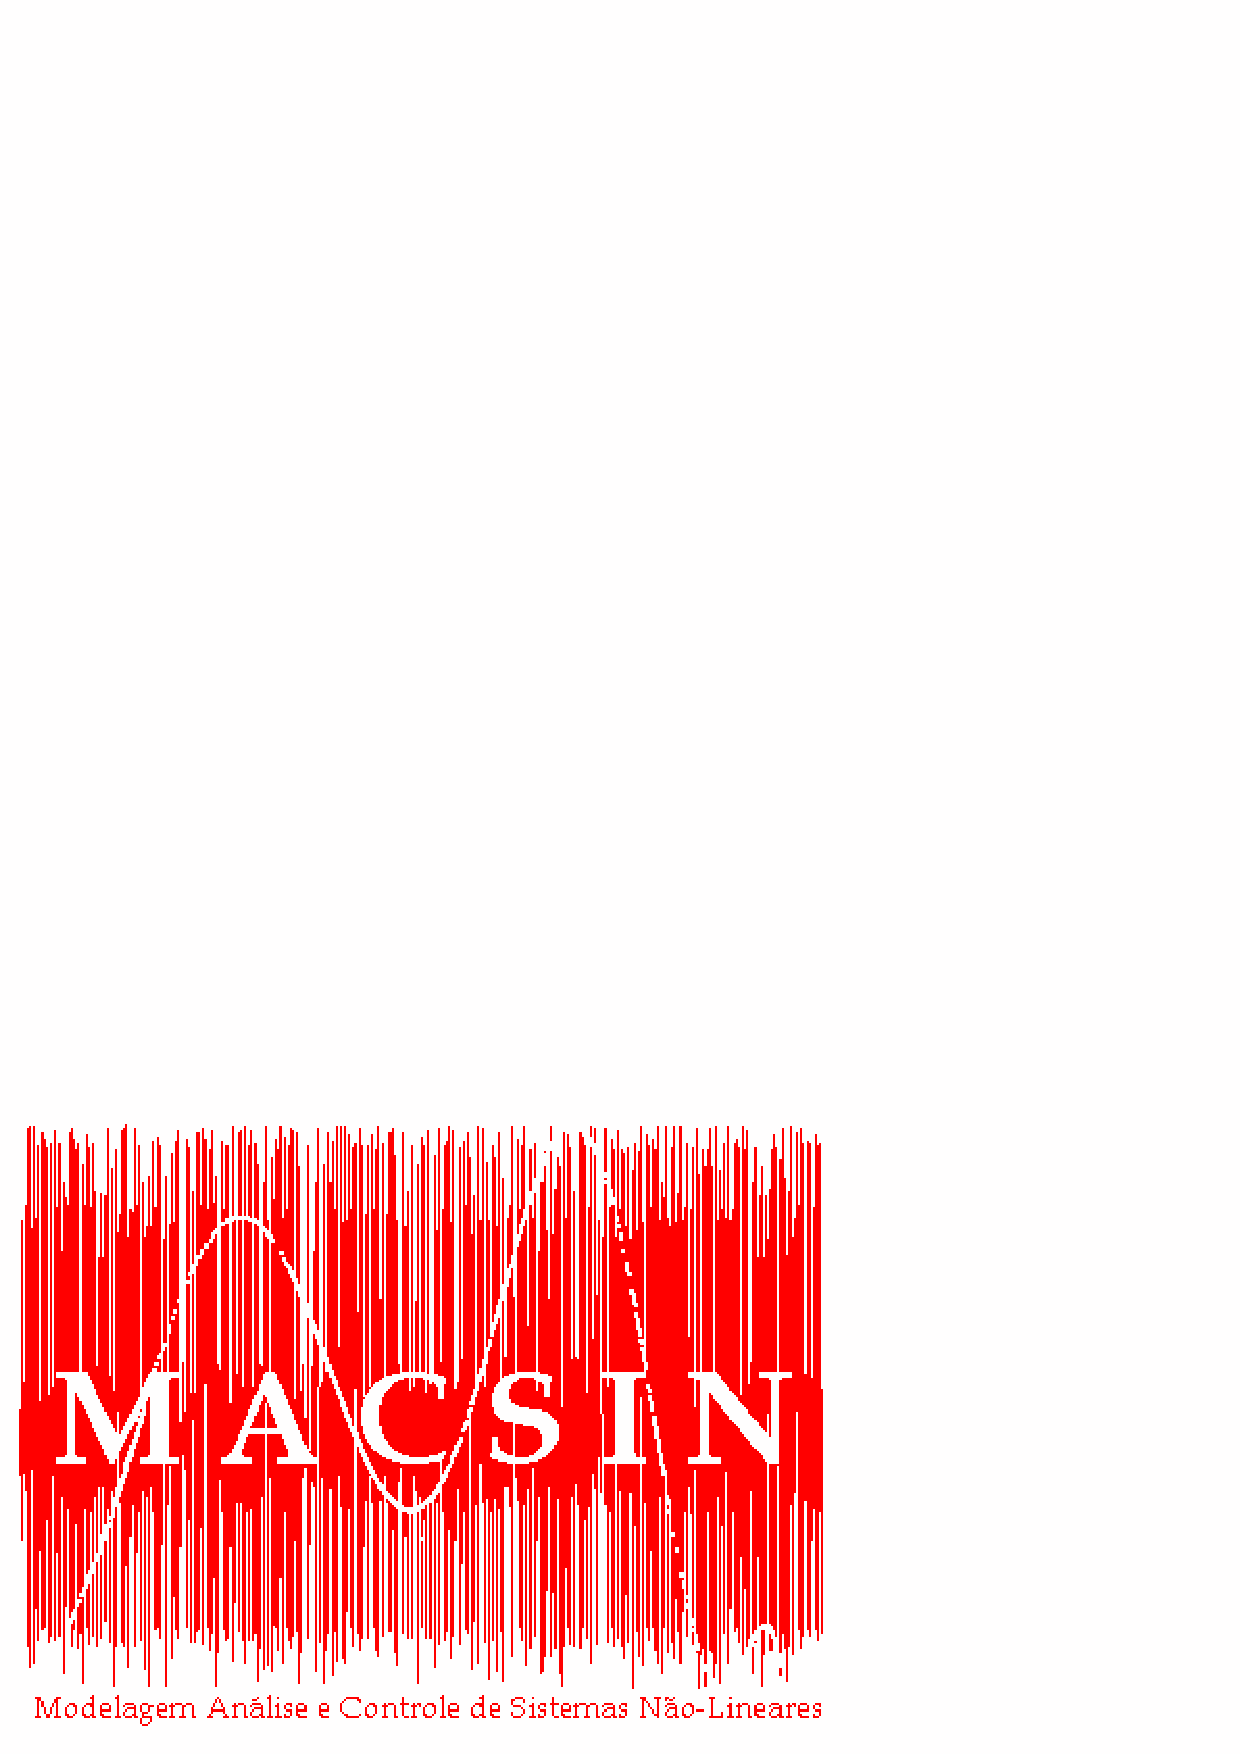
\includegraphics[scale=0.3,trim=0mm 3mm 65mm 188mm,clip=true]{figuras/macsin.pdf}
\end{flushright}
\end{minipage}
\end{figure}
%--------------------------------------------------------------------

%Título
%--------------------------------------------------------------------
\vspace{3cm}
\begin{center}
	
%Autor
%--------------------------------------------------------------------
{\normalsize Luís Henrique dos Santos}\\[4cm]
\thickhrulefill
\par\nobreak
\vspace*{10\p@}%
\hrule
\vspace*{10\p@}%
{\bf \normalsize \bfseries {IDENTIFICAÇÃO DE MODELOS DE HAMMERSTEIN \\MULTIVARIÁVEIS COM NÃO LINEARIDADES ESTÁTICAS OU\\ QUASE ESTÁTICAS FORTES}}
\vspace*{10\p@}%
\hrule
\vspace*{40\p@}%
%--------------------------------------------------------------------
\end{center}
%--------------------------------------------------------------------

\vspace{7cm}

%--------------------------------------------------------------------
%Cidade e Data
%--------------------------------------------------------------------
\centering{\normalsize Belo Horizonte \\ 
	2024} 
%\centerline{\large 2024}
%--------------------------------------------------------------------
\end{titlepage}
